El primer concepto que deberiamos fundar en esta explicacion es el de ``Espectro Electromagnético'', esto podemos verlo de la siguiente manera:  \\${ }$\\
Cuando los electrones se mueven, crean ondas electromagnéticas que se propagan por el espacio (incluso el vacio). Estas ondas fueron predichas por James Maxwell en 1865 y observadas por Heinrich Hertz en 1887. El número de oscilaciones por segundo de una onda es llamado \textit{frecuencia} ($f$) es medida en $Hz.$ La distancia entre dos crestas (máxima/mínima) es llamada longitud de onda ($\lambda$).


\section*{Transmisión Inalámbrica}
No implica un enlace fisico entre dos o mas dispositivos. Las señales inalambricas se extienden por el aire y son recibidas e interpretadas por antenas, estas convierten los datos y los extiende por todo su rango de frecuencias. Mientras que el receptor en el otro extremo recibe las señales y las convierte en señales digitales. \\ ${ }$\\
Cuando una antena tiene el tamaño apropiado y está conectado a un circuito electrico, las ondas electromagnéticas pueden transmitirse de manera eficiente y ser recibidas por un receptor a cierta distancia. Todas las comunicaciones inalambricas se basan en este principio.
\subsection*{Radio Transmisión}
Las radio frecuencias (RF) son faciles de generar, pueden viajar largas distancias y penetrar edificios, son ampliamente utilizadas en conexiones de interiores y exteriores. Las ondas de radio son omnidireccionales, esto significa que viajan en todas las direcciones de la fuente. Eso quiere decir que el transmisor no necesariamente debe estar alineado (físicamente). 
\\ Un ejemplo de el uso de RF lo tenemos en los años 70s. Cuando \textbf{GM} decidió equipar autos con frenos asistidos por computadora, mientras que otra empresa empezo a usar un nuevo sistema de radio y estos lo usaban para comunicarse, por lo que los autos que contaban con este sistema de frenado constantemente frenaban. Esto debido a la antena colocada en el autos. Ya que estas son dependientes de las frecuencias. \\ ${ }$ \\
A menor frecuencia las ondas de radio traspasan obstaculos con mas facilidad pero el alcance es notoriamente bajo desde la fuente, a esta atenuacion se le llama \textbf{perdida de ruta.} En todas las frecuencias las ondas de radio estan sujetas a interferencia de motores u otros equipos electricos.

\begin{figure}[H]
\centering
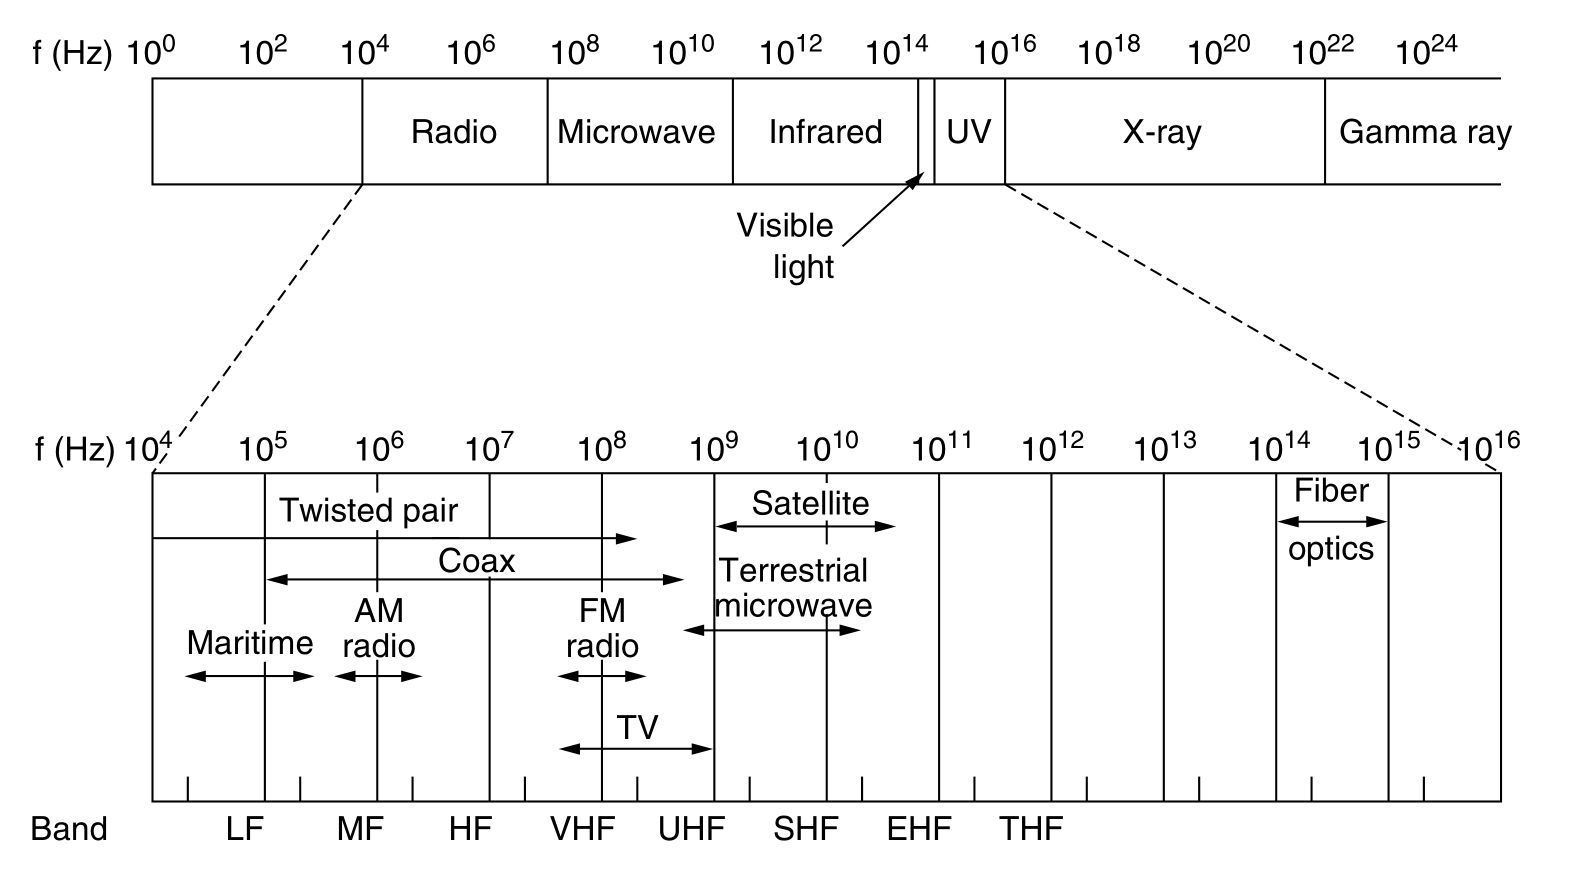
\includegraphics[scale=0.6]{ESPECTRO.png}
\caption{Esquema comercial del espectro electromagnético. \textit{(Página 107, Tanenbaum 5ta Edición)}}
\end{figure}
En VLF, LV, y MF las ondas de radio siguen el suelo. Estas ondas pueden ser detectadas a 1000 Km a frecuencias bajas. Estas ondas de radio pasan a travez de edificios facilmente lo que las hace ideal para interiores, el problema es su bajo ancho de banda. \textbf{(a)}
\\
En las bandas HF y VHF, las ondas de tierra tienden a ser absorbidas por la tierra. Sin embargo, las ondas que alcanzan la ionosfera, una capa de partículas cargadas que circundan la tierra a una altura de 100 a 500 km, son refractadas por ella y enviadas de regreso a la tierra. \textbf{(b)}

\begin{figure}[H]
\centering
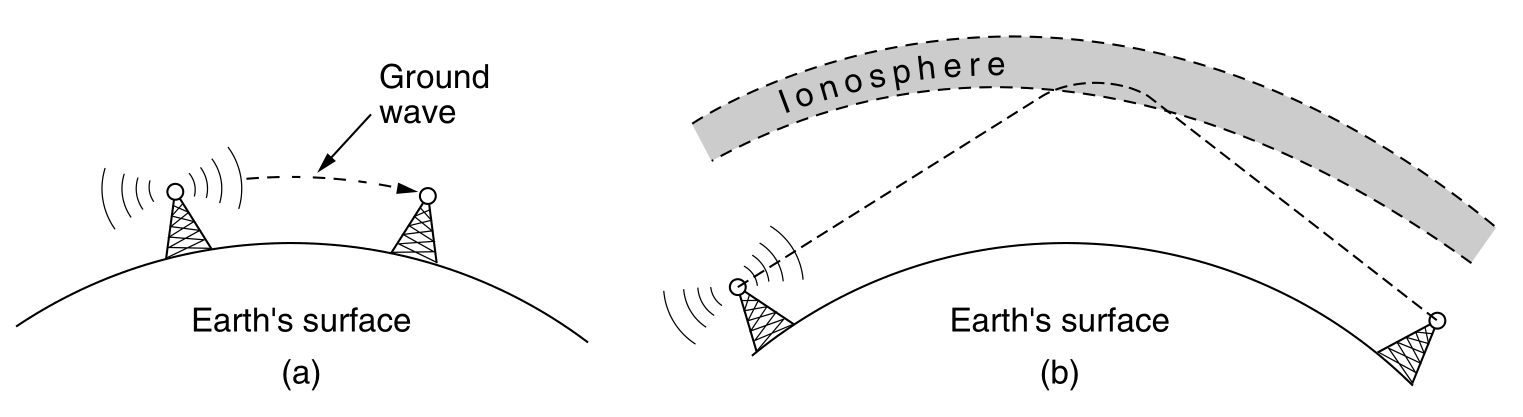
\includegraphics[scale=0.6]{ANTENA.png}
\caption{Formas de tranmisión con Antenas. \textit{(Página 110, Tanenbaum 5ta Edición)}}
\end{figure}

\subsubsection*{Propagación de Ondas de Radio}

Para instalar una red inalámbrica y, en particular, ubicar los puntos de acceso a fin de obtener el máximo alcance posible se deben conocer algunos datos con respecto a la propagación. Las ondas de radio (RF) se propagan en línea recta en varias direcciones al mismo tiempo. En cualquier otro medio la señal se volverían mas debil debido a la reflexión, la refracción, la difracción y la abstracción.

\subsubsection*{Transmisión y recepción}
Una onda de radio se origina cuando una partícula cargada, se excita a una frecuencia situada en la zona de radiofrecuencia (RF) del espectro electromagnético. Otros tipos de emisores que caen fuera de la gama RF son rayos gammas, rayos X, infrarrojos, ultravioleta y luz. Cuando la onda de radio actúa sobre un conductor eléctrico, induce en el un movimiento de la carga eléctrica que puede ser transformado en señales de audio u otros tipos de información.

\subsubsection*{Reflexión de Ondas de Radio}

Cuando una onda de radio choca con un obstáculo, parte o la totalidad de la onda se refleja y se observa una pérdida de la intensidad. \\ ${ }$ \\ Por definición, una onda de radio es susceptible de propagarse en varias direcciones. Despues de reflejarse varias veces, una señal de origen puede llegar a una estación o punto de acceso despues de tomar muchas rutas. Por esto, las tarjetas Wi-Fi usan 2 antenas por emisor. Mediante un controlador que cambia inmediatamente de una antena a otra.


\begin{center}
\begin{tabular}{*2l}
\toprule
Ventajas &   {} \\
\midrule\hspace{-0.4cm} \makecell{$\bigstar$Es barato donde el cable\\no puede instalarse facilmente.}    \\
$\bigstar$Atraviesa Paredes   \\
$\bigstar$Son omnidirecionales  \\
\bottomrule
\end{tabular}
\quad
\begin{tabular}{*2l}
\toprule
Desventajas &   {} \\
\midrule
\hspace{-1.7cm} \makecell{$\spadesuit$No es práctico para\\ velocidades altas.}  \\
\makecell{$\spadesuit$Esta sometido a interferencias\\ (aficionados, militares,etc.)}\\
\bottomrule
\end{tabular}
\end{center}

\subsection*{Transmisión Microonda}

Por encima de los 100$Mhz$ las ondas viajan en línea recta y en consecuencia, se puede enfocar con un haz estrecho. Al concentrar toda la energía en un pequeña haz por medio de una antena parabólica se obtiene una relación señal-ruido mucho mas alta pero las transmisiones y receptores deben estar alineados. \\${ }$\\
Puesto que las microondas viajan en linea recta, si las torres estan separadas, la Tierra se interpondrá en el camino. Por ende se necesitan repetidores periódicos. Entre mas altas las torres mas separadas pueden estar. Existen dos tipos de microondas:
\begin{itemize}
\item \textbf{Microondas Terrestres:} Suelen utilizarse antenas parabólicas. Para conexiones de larga distancia se utilizan conexiones intermedias punto a punto entre antenas parabólicas. Se suelen utilizar en sustitución del coaxial ya que necesitan menos repetidores y amplificadores.
\item \textbf{Microondas Satelitales:} Estas basicamente lo que hacen es retransmitir información, se usan como enlace entre dos o mas transmisores/receptores terrestres denominados estaciones base.
\end{itemize}

%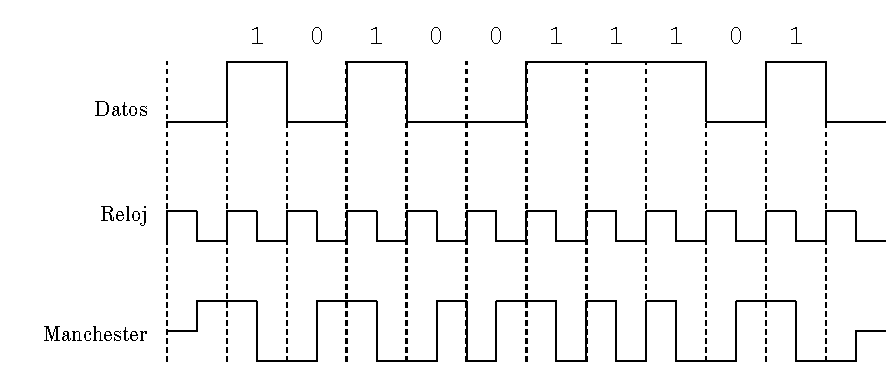
\includegraphics[page=1,scale=0.9]{Manchester.pdf}


%\begin{figure}[ht!]
%\centering
%\scalebox{.5}{
%\import{images/}{HDLCim.pdf_tex}
%}
%\caption{Ejemplo de la Trama.}
%\end{figure}
